\subsubsection{Les cases}
La carte du monde est constituée de cinq types de cases hexagonales : les salles infos, les salles de TD, les amphithéâtres, le restaurant et les extérieurs.\\
Il y a de un à trois restaurants selon le type de map choisi, la moitié des cases sont des extérieurs, et le reste est réparti équitablement entre les autres types.\\
Le coût de déplacement de base depuis une case est de 1, sauf pour le restaurant où il est de 2. Ce coût peut varier en fonction du peuple de l'unité se déplaçant.
\begin{figure}[!h]
\centering
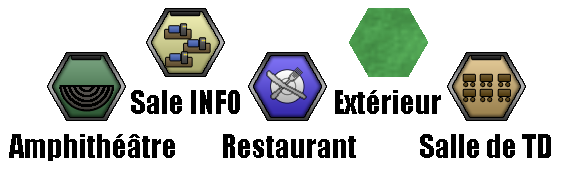
\includegraphics[width=.7\textwidth]{Parties/Images/Terrains.png}
\caption{Les différentes cases, comme elles sont représentées dans le jeu}
\label{fig:Terrains}
\end{figure}


\subsubsection{Les différents types de jeu}
Il existe trois cartes différentes :
\begin{itemize}
\item Démo : 2 joueurs, 6*6 cases, 5 tours, 4 unités par joueur.
\item Petite : 2 joueurs, 10*10 cases, 20 tours, 6 unités par joueur.
\item Normale : 2 joueurs, 14*14 cases, 30 tours, 8 unités par joueur.
\end{itemize}